\documentclass[11pt]{article}
\usepackage[margin=0.7in]{geometry}
\usepackage{amsmath,amssymb}
\usepackage{enumitem}
\usepackage{tikz}
\usepackage{pgfplots}
\pgfplotsset{compat=1.18}
\usepackage{fancyhdr}
\usepackage{parskip}
\setlist[enumerate]{leftmargin=*, itemsep=6pt}
\pagestyle{fancy}
\fancyhf{}
\fancyfoot[L]{\small\textit{en}Vision\textsuperscript{\textregistered} Algebra 2}
\fancyfoot[C]{\small 3-1 Lesson Quiz, short form}
\fancyfoot[R]{\small\thepage}
\renewcommand{\headrulewidth}{0pt}
\newcommand{\choice}[1]{\tikz[baseline=-0.6ex]\node[draw, circle, inner sep=0.6pt, minimum size=3.3mm, font=\scriptsize\bfseries] {#1};\;}
\newcommand{\checkbox}{$\square$\;}
\pgfplotsset{quizgrid/.style={
  axis lines=middle, grid=both, grid style={gray!45},
  ticklabel style={font=\scriptsize, fill=white, inner sep=1pt},
  xlabel={$x$}, ylabel={$y$}, axis line style={thick}, clip=true}}

\begin{document}

\noindent\textbf{Name}\; \rule{6cm}{0.4pt} \hfill Period \rule{1.2cm}{0.4pt} \quad Date \rule{2.2cm}{0.4pt}

\vspace{4pt}\noindent\rule{\textwidth}{0.6pt}

\vspace{2pt}\noindent{\LARGE\textbf{3-1 \; Lesson Quiz: Graphing Polynomial Functions}} \hfill {\small short form}

\vspace{4pt}\noindent\rule{\textwidth}{0.6pt}

\noindent{\small Question numbers are the Savvas quiz numbers; questions 1 and 5 are not on this form.}

\vspace{2pt}
% Savvas item 2
\textbf{2.} Use the leading coefficient and degree of the polynomial function $f(x)=x^3-7x^2+10x$ to determine the end behavior of its graph. Select \textbf{all} the true statements.

\vspace{4pt}
\begin{itemize}[leftmargin=1.2em, itemsep=2pt]
\item[] \checkbox \textbf{A.} As $x\to\infty$, $y\to\infty$.
\item[] \checkbox \textbf{B.} As $x\to\infty$, $y\to-\infty$.
\item[] \checkbox \textbf{C.} As $x\to\infty$, $y\to0$.
\item[] \checkbox \textbf{D.} As $x\to-\infty$, $y\to\infty$.
\item[] \checkbox \textbf{E.} As $x\to-\infty$, $y\to-\infty$.
\end{itemize}

\vspace{4pt}
Degree: \rule{1.2cm}{0.4pt} \qquad Leading coefficient: \rule{1.2cm}{0.4pt}

\vspace{4pt}\noindent\rule{\textwidth}{0.4pt}

\vspace{6pt}
% Savvas item 3
\begin{minipage}[t]{0.5\textwidth}
\textbf{3.} The graph of a function $f$ is shown. Use the graph to estimate all turning points. Select \textbf{all} $x$-values that are turning points of $f$.

\vspace{4pt}
\begin{itemize}[leftmargin=1.2em, itemsep=2pt]
\item[] \checkbox \textbf{A.} $-3$
\item[] \checkbox \textbf{B.} $0$
\item[] \checkbox \textbf{C.} $4$
\item[] \checkbox \textbf{D.} $-1.5$
\item[] \checkbox \textbf{E.} $1$
\item[] \checkbox \textbf{F.} $-1$
\item[] \checkbox \textbf{G.} $1.5$
\end{itemize}
\end{minipage}\hfill
\begin{minipage}[t]{0.46\textwidth}
\vspace{-4pt}
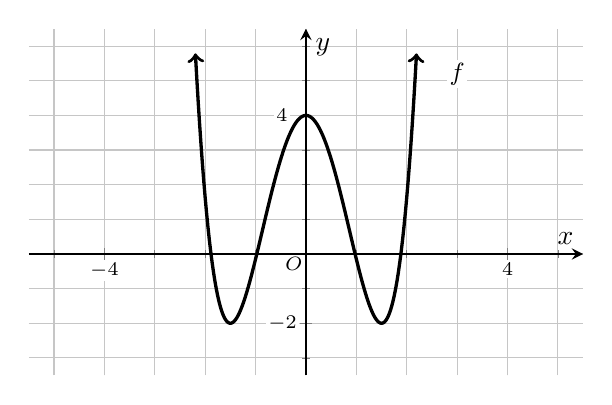
\begin{tikzpicture}
% TE window x[-5,5], y[-3,6], unit grid, x labels -4,4, y labels -2,4, O at the origin; the "4" label is drawn left of the maximum (0,4).
\begin{axis}[quizgrid, xmin=-5.5, xmax=5.5, ymin=-3.5, ymax=6.5,
  xtick={-4,4}, ytick={-2}, minor xtick={-5,...,5}, minor ytick={-3,...,6},
  minor grid style={gray!45}, x=0.64cm, y=0.44cm]
\addplot[very thick, <->, domain=-2.194:2.194, samples=160] {32/27*x^4-16/3*x^2+4};
\node[font=\scriptsize, fill=white, inner sep=1pt, anchor=east] at (axis cs:-0.3,4) {$4$};
\node[font=\scriptsize, fill=white, inner sep=1pt, anchor=north east] at (axis cs:0,0) {$O$};
\node[font=\small, fill=white, inner sep=1pt] at (axis cs:3,5.2) {$f$};
\end{axis}
\end{tikzpicture}
\end{minipage}

\vspace{4pt}\noindent\rule{\textwidth}{0.4pt}

\vspace{6pt}
% Savvas item 4
% Corrected from a2_3-1_TE.tex lines 771 and 773, which print the intervals (-\infty,1/3), (3,\infty) and (1/3,3):
% f'(x) = -3x^2+10x-2 = 0 at x = (5 -+ sqrt 19)/3, about 0.214 and 3.120, so f is not decreasing on all of (-\infty,1/3)
% (f'(0.25) > 0). The turning points are named a and b instead; the answers are unchanged.
\begin{minipage}[t]{0.52\textwidth}\raggedright
\textbf{4.} Use the graph of the polynomial function \mbox{$f(x)=-x^3+5x^2-2x-8$} to complete the sentences. Its turning points are at $x=a\approx0.21$ and $x=b\approx3.12$.

\vspace{4pt}
Word bank: decreasing; increasing; negative; positive.

\vspace{8pt}
$f$ is \rule{2.4cm}{0.4pt} on the intervals $(-\infty,a)$ and $(b,\infty)$.

\vspace{8pt}
$f$ is \rule{2.4cm}{0.4pt} on the intervals $(-1,2)$ and $(4,\infty)$.

\vspace{8pt}
$f$ is \rule{2.4cm}{0.4pt} on the interval $(a,b)$.

\vspace{8pt}
$f$ is \rule{2.4cm}{0.4pt} on the intervals $(-\infty,-1)$ and $(2,4)$.
\end{minipage}\hfill
\begin{minipage}[t]{0.45\textwidth}
\vspace{-4pt}
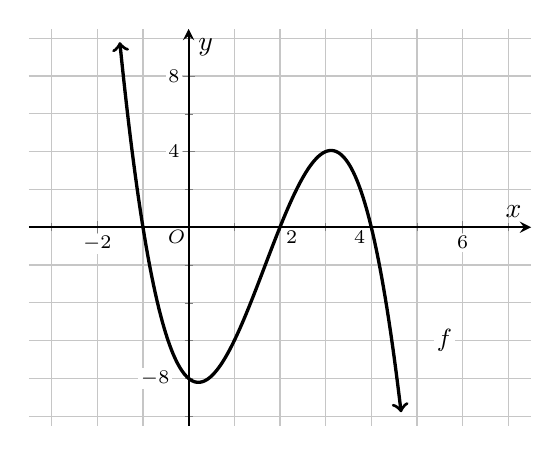
\begin{tikzpicture}
% TE window x[-3,7], y[-10,10]; x unit grid, labels -2,2,4,6; y grid 2, labels -8,4,8; O at the origin.
% The 2 and 4 labels sit beside the zeros on the side the curve does not cross; -8 sits left of where the curve hugs y = -8.
\begin{axis}[quizgrid, xmin=-3.5, xmax=7.5, ymin=-10.5, ymax=10.5,
  xtick={-2,6}, ytick={4,8}, minor xtick={-3,...,7}, minor ytick={-10,-8,...,10},
  minor grid style={gray!45}, x=0.58cm, y=0.24cm]
\addplot[very thick, <->, domain=-1.507:4.653, samples=160] {-x^3+5*x^2-2*x-8};
\node[font=\scriptsize, fill=white, inner sep=1pt, anchor=north west, xshift=1pt] at (axis cs:2,0) {$2$};
\node[font=\scriptsize, fill=white, inner sep=1pt, anchor=north east, xshift=-1pt] at (axis cs:4,0) {$4$};
\node[font=\scriptsize, fill=white, inner sep=1pt, anchor=east] at (axis cs:-0.35,-8) {$-8$};
\node[font=\scriptsize, fill=white, inner sep=1pt, anchor=north east] at (axis cs:0,0) {$O$};
\node[font=\small, fill=white, inner sep=1pt] at (axis cs:5.6,-6) {$f$};
\end{axis}
\end{tikzpicture}
\end{minipage}

\vfill
\noindent\textbf{Scoring:} Question 2 and Question 3 are 10 points each. Question 4 is a bonus of up to 5 points. Total out of 20.

\newpage
\noindent{\LARGE\textbf{3-1 Lesson Quiz, short form: answer key}}

\vspace{4pt}\noindent\rule{\textwidth}{0.6pt}

\begin{enumerate}
\item[\textbf{2.}] \textbf{A, E.} $f(x)=x^3-7x^2+10x$ is already in standard form: degree 3 (odd), leading coefficient 1 (positive), so the ends point opposite ways and the right end goes up: as $x\to\infty$, $y\to\infty$; as $x\to-\infty$, $y\to-\infty$. Savvas quiz item 2, DOK 1, Skills Review and Practice A73 (taught by Example 2). \textbf{10 points:} 5 for each correct box; take 5 off for each wrong box (B, C or D), not below 0. The degree and leading-coefficient line is the student's work and is not scored.
\item[\textbf{3.}] \textbf{B, D, G} ($x=0$, $x=-1.5$, $x=1.5$). The graph changes from increasing to decreasing at the relative maximum $(0,4)$ and from decreasing to increasing at the relative minimums near $(-1.5,-2)$ and $(1.5,-2)$. Choices E and F ($\pm1$) are $x$-intercepts, not turning points; C ($4$) is the $y$-value of the maximum. Savvas quiz item 3, DOK 2, A73 (taught by Example 3). \textbf{10 points:} 3 for each correct box plus 1 for no wrong box; take 3 off for each wrong box, not below 0.
\item[\textbf{4.}] \textbf{decreasing; negative; increasing; positive.} Increasing/decreasing: read left to right between the turning points at $x=a=\tfrac{5-\sqrt{19}}{3}\approx0.21$ and $x=b=\tfrac{5+\sqrt{19}}{3}\approx3.12$. Positive/negative: above or below the $x$-axis between the zeros $-1$, $2$, $4$. Savvas quiz item 4, DOK 2, A73 (Example 3 for increasing/decreasing; the packet's Practice for positive/negative). \textbf{Bonus 5:} 1 point per sentence, plus 1 for all four. \emph{Teacher note:} the Savvas quiz prints the intervals as $\left(-\infty,\tfrac13\right)$, $(3,\infty)$ and $\left(\tfrac13,3\right)$, which are not exact ($f$ is already increasing at $x=0.25$); this form names the turning points $a$ and $b$ instead. The answers are the same.
\end{enumerate}

\textbf{Graphs.} Question 3 is redrawn from the TE description (W-shaped quartic, relative maximum $(0,4)$, relative minimums at $(\pm1.5,-2)$, $x$-intercepts near $\pm1$ and $\pm2$; the curve drawn is $y=\tfrac{32}{27}x^4-\tfrac{16}{3}x^2+4$, whose intercepts are $\pm0.98$ and $\pm1.88$). Question 4 is the given function on the TE window; its turning points are at $x\approx0.21$ (minimum about $-8.21$) and $x\approx3.12$ (maximum about $4.06$); the TE's figure note says ``near $(\tfrac13,-8.3)$'' and ``at $(3,4)$''.

\textbf{Items left off this form} (available for a retake or Form B): Savvas item 1, ``Which statement is true of $f(x)=x^2+6x^3-4+2x^5$?'' (answer C, the graph has exactly one $x$-intercept; DOK 2, A73; it needs a graph or table of a quintic, and choice D, ``increasing for all real numbers,'' is false only on a tiny interval, about $-0.11<x<0$, that a hand sketch cannot show); Savvas item 5, the water-tank $y$-intercept, $y=1.15x^3-0.1x^2+2$ (answer: 2; volume of water; turned on; DOK 2, A73; taught by Example 5, which this lesson cuts).

\textbf{IXL replacement:} SmartScore 70 or above on XMK and XJU replaces this quiz with 20/20.

\end{document}
